%% ****** Start of file apsguide4-1.tex ****** %
%%
%%   This file is part of the APS files in the REVTeX 4.1 distribution.
%%   Version 4.1r of REVTeX, August 2010.
%%
%%   Copyright (c) 2009, 2010 The American Physical Society.
%%
%%   See the REVTeX 4.1 README file for restrictions and more information.
%%
\documentclass[10pt]{article}


\usepackage{color}
\usepackage[latin9]{inputenc}
\usepackage{mathrsfs,amsmath}

\usepackage{graphicx}
\usepackage{float}
\usepackage{amsfonts}%
\usepackage[titletoc]{appendix}
\usepackage{amssymb}
\usepackage{braket}
\usepackage{bm}
\usepackage{authblk}
\newcommand{\mb}[1]{\bm{#1}}
\usepackage[T1]{fontenc}




\usepackage{hyperref}
\newcommand{\footremember}[2]{%
	\footnote{#2}
	\newcounter{#1}
	\setcounter{#1}{\value{footnote}}%
}
\newcommand{\footrecall}[1]{%
	\footnotemark[\value{#1}]%
} 


\def\Nabla{\bm{\nabla}}
\def\bm{\mathbf}
\def\curl{\Nabla\times}
\def\div{\Nabla\cdot}
\def\lap{\Delta}
\def\vlap{\Delta}
\def\x{\hat{e}_{x}}
\def\y{\hat{e}_{y}}
\def\z{\hat{e}_{z}}
\def\p{\partial}
\def\h{\hat}
\DeclareMathOperator{\Tr}{Tr}


\title{Slow Light via Resonant-tunneling Induced Transparency in Quantum Well Heterostructures}
\author{Petar Tzenov}
\author{Christian Jirauschek}
\affil{Institute for Nanoelectronics, Technical University of Munich, D-80333 Munich, Germany}
\date{}
\setcounter{Maxaffil}{0}
\renewcommand\Affilfont{\itshape\small}
\bibliographystyle{ieeetr}

\usepackage{chngcntr}
\counterwithout{figure}{section}
\begin{document}
\maketitle

\section{Introduction}
We present a theoretical and computational investigation of the possibility of achieving slow and superluminal terahertz light by exploiting the tunneling induced transparency effect in suitably engineered quantum well heterostructure devices \cite{borges2012tunneling}. Our calculations show that for optimal system parameters a slow-down factor larger than 10 could be possible and we also derive necessary conditions for achieving superluminal light.  

\section{Model}
In our model, we consider a periodic structure consisting of two quantum wells per module, in which the lowest energy eigenstate of module I,  couples via resonant tunneling to the excited state of the next period, i.e. II, and the resulting triplet $\ket{s},\ket{e}$ and $\ket{g}$ forms a $\Lambda-$type system (see Fig. \ref{fig:img01}a). At optimal bias, the electron levels spanning an inter-module barrier energetically align to form a strongly coupled pair of dressed states, which results in splitting of the absorption spectrum of the sample. Such an effect is familiar to the quantum cascade laser community \cite{faist1997controlling,burghoff2014terahertz}, however, to the extend of our knowledge, until this point it had not yet been considered in the context of producing slow light.

For our investigation we couple a Schr�dinger-Poisson, ensemble Monte-Carlo \cite{jirauschek2014modeling} and Maxwell-Bloch simulation codes, which enables us to self-consistently design and analyze various systems with the desired properties. Simulations with suitably chosen, but still realistic, parameters show the possibility of a group velocity delay by a factor of 11.6 with respect to the velocity of light in vacuum. 
\section{Results}
\begin{figure}[h!]
	\centering
	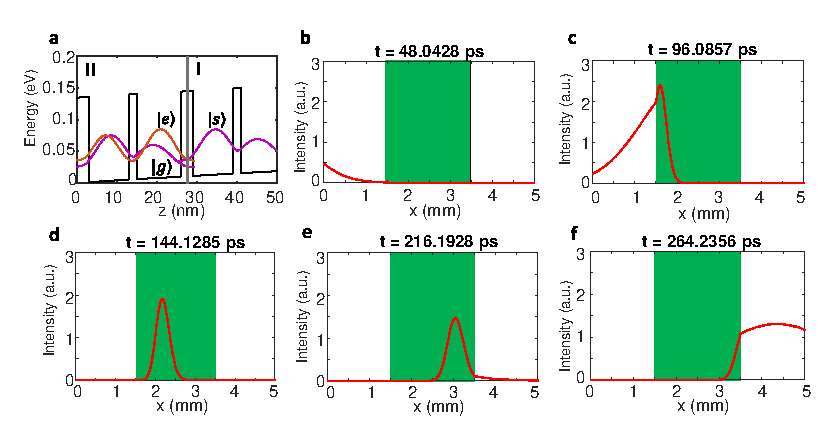
\includegraphics[scale=0.8]{SLOWLIGHT.eps} 
	\label{fig:img01}
\end{figure}
Fig. \ref{fig:img01}b-e illustrates preliminary results from Maxwell-Bloch equation simulations for the propagation of a weak 30 picosecond pulse through a 2 mm long active region (shaded area), in the ideal case of vanishing $\ket{s}\leftrightarrow\ket{g}$ dephasing. The propagation direction is along the $x$-axis whereas the heterostructure growth direction along $z$. We have also neglected the dependence of the electric field on the transverse $y$-direction.

 In Fig. \ref{fig:img01}c-d we can observe a strong compression of the pulse upon its incidence on the active region, followed by reduction in its overall intensity due to dephasing. Upon leaving the interaction medium, the pulse is again broadened, Fig. \ref{fig:img01}e-f, as outside of the shaded area it's group velocity is equal to the velocity of light in the host material. Our calculations reveal a group refractive index $n_g\approx 11.6$, however we believe that better values can be achieved with a more careful parameter study \cite{boller1991observation}. 

\bibliography{literature.bib}

\end{document}

